%1. Intro White-box, overview of analysis
%2. Explaining some analyzing strats that are out there
%3. VaRA, explain what vara does roughly (Regions)
%4. Vara TS Experiment explain
%5  TEF Report and how we evaluate them
%6. Using data to build multiple perf-influcence models


\colorlet{punct}{red!60!black}
\definecolor{background}{HTML}{EEEEEE}
\definecolor{delim}{RGB}{20,105,176}
\colorlet{numb}{magenta!60!black}
\lstdefinelanguage{json}{
    basicstyle=\normalfont\ttfamily,
    numbers=left,
    numberstyle=\scriptsize,
    stepnumber=1,
    numbersep=8pt,
    showstringspaces=false,
    breaklines=true,
    frame=lines,
    backgroundcolor=\color{background},
    literate=
     *{0}{{{\color{numb}0}}}{1}
      {1}{{{\color{numb}1}}}{1}
      {2}{{{\color{numb}2}}}{1}
      {3}{{{\color{numb}3}}}{1}
      {4}{{{\color{numb}4}}}{1}
      {5}{{{\color{numb}5}}}{1}
      {6}{{{\color{numb}6}}}{1}
      {7}{{{\color{numb}7}}}{1}
      {8}{{{\color{numb}8}}}{1}
      {9}{{{\color{numb}9}}}{1}
      {:}{{{\color{punct}{:}}}}{1}
      {,}{{{\color{punct}{,}}}}{1}
      {\{}{{{\color{delim}{\{}}}}{1}
      {\}}{{{\color{delim}{\}}}}}{1}
      {[}{{{\color{delim}{[}}}}{1}
      {]}{{{\color{delim}{]}}}}{1},
}


%************************************************
\section{White-box Model}\label{ch:Whitebox}
%************************************************
A black-box analysis is very useful for systems where we do not have access to the source code, but if we do, we take advantage of this additional information,
by using a white-box analysis. 
While a black-box analysis measures the time we spend inside the system from start to finish and collects measurements while doing so, 
a white-box analysis archives a higher level of granularity by using a different algorithm to determine how much time we spend in each feature.

Afterward built a {\perfInfluenceModel} out of the data we collected using the white-box analysis.

\begin{figure}[h]
    \centering
    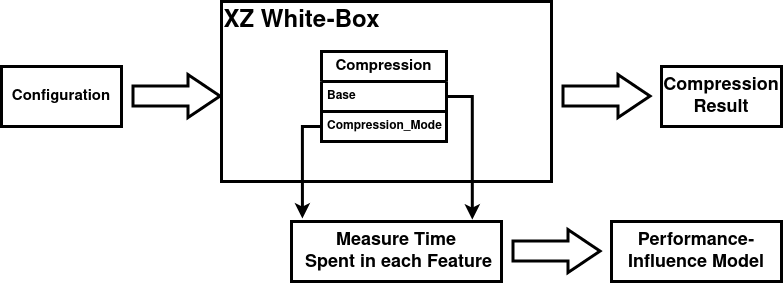
\includegraphics[scale=0.55]{gfx/whitebox_2.png}
    \caption{Process of using a black-box analysis to build a \perfInfluenceModel for \textit{XZ}.}
    \label{fig:WBxz}
\end{figure}

Using a white-box analysis, we now analyze the example system from \autoref{fig:xz}. 
In \autoref{fig:WBxz}, we have access to the source code of \textit{XZ}; 
our first step is to manually analyze the code and find the variables that implement configurability inside the system. 
In this example, we found the feature \textit{Base} and \textit{compression\_mode}. 
During compression, we use our white-box analysis to measure the time spent by \textit{XZ} in the different features. 
This example measures the time spent in $Base$ and $Compression\_Mode$. 
After the system finished the process, we collected all the measurements, which we then used to build a {\perfInfluenceModel} for this configuration.

In \autoref{analyzing-strats}, we explain the current state-of-the-art strategies used to analyze systems using white-box. 
Subsequently, in \autoref{VaRA} we introduce VaRA, the analyzing tool we use, and its underlying principles. 
In \autoref{trace-event}, we explain how to build the {\perfInfluenceModel} using the white-box data.

\subsection{Strategies}\label{analyzing-strats}
When analyzing systems using a white-box approach, different strategies have been introduced. 
In this chapter, we explain three different strategies, \textsc{ConfigCrusher} and \textsc{Comprex}, 
both model configurability on a feature level, whereas Weber et al. introduce a strategy that models configurability on a method level.

Velez et al. introduced us to \textsc{ConfigCrusher} \cite{ConfigCrusher}, 
a white-box analysis that uses static data-flow analysis to see how features influence variables and the control flow of the system. 
In addition, ConfigCrusher leverages three insights about configurable systems from previous works, namely irrelevance, orthogonality, 
and low interaction degree. They use irrelevance to identify features relevant to the system's data flow, 
reducing the number of configurations required to analyze the system. They use orthogonality to identify features that do not interact with each other and, 
therefore, can be measured together. Since only a few features interact, 
\textsc{ConfigCrusher} focuses on the configurations with interacting features to reduce the number of configurations to be analyzed. 
From these findings, two techniques are developed, namely compression and composition. 
They use compression to reduce the number of configurations required to analyze the system by simultaneously analyzing regions that are independent of each other 
so that they can use a single configuration to analyze different features. 
Whereas composition takes advantage of the fact that {\perfInfluenceModel} can be built compositionally by building a performance-influcence model 
for each region separately and then assembling all local {\perfInfluenceModel} into one model for the entire system.
After using the data-flow analysis to generate a control flow graph and a statement influcence map, which maps statements to the configuration options 
that influence that statement.
Afterward, they use both the control flow graph and statement influcence map to instrument the regions in the system that correspond to features and execute
the instrumented system to track execution time of each feature. From these measurements, they build the {\perfInfluenceModel} for the system.

Velez et al. introduced \textsc{Comprex} \cite{Comprex}, an approach that builds on \textsc{ConfigCrusher} 
but uses an iterative dynamic taint analysis instead of static analysis to determine how and to what extent features affect the control flow of the given system.
By doing so, they identify which code regions are influenced by which configurations and, during execution measure the time spent in these regions to then build 
the {\perfInfluenceModel}.

Compared to \textsc{ConfigCrusher} and \textsc{Comprex}, Weber et al. 
\cite{White-box-Profiling} uses a profiling approach to generate performance-influence models that analyze configurability on a method level. 
To achieve this, they first used \textsc{JProflier}, a coarse-grained profiler, 
to learn a performance-influence model for every method that has been learned successfully. To identify the hard-to-learn methods, 
they use filtering techniques and then \textsc{KIEKER}, a fine-grained profiler, to learn these methods. At the end, for each method, they
obtain a {\perfInfluenceModel} that shows how strong each feature influences the performance of that method.


\subsection{VaRA}\label{VaRA}
To analyze the system we are interested in, we use VaRA, a framework for analyzing configurable software systems that is built on LLVM.
In addition, we use the VaRA Tool Suite\footnote{Visited at 14.03.2022 \url{https://vara.readthedocs.io}}, which provides us with a framework that supports
us when analyzing configurable systems using VaRA.
. 
The purpose of VaRA is to provide various analyses for systems where the user only needs to focus on the high-level conceptual information of the 
system, while VaRA handles the low-level-details. 
Since VaRA is built on top of LLVM, it is able to analyze systems written in languages that can be compiled by LLVM, such as C, C++ or Rust. 

VaRA is able to perform a static analysis to analyze the source code directly. The way VaRA does that is by analyzing the
abstract syntax tree of the system and locate the if-blocks along with variables that represent features together they form 
feature regions. Then, VaRA instruments the binary so that we are able to track the time spent in each feature region
during the dynamic analysis when we run the binary. \cite{VaRA-Flo}

\lstset{style=myStyle}
\begin{minipage}{\linewidth}
\begin{lstlisting}[caption={Feature region example},language=C++,label={alg:Vara_feature_regions},escapechar=|]
void encrypt() {
    bool Encryption; //Feature Variable | \label{line:encryption_feature_variable} |
    assign_feature(Encryption); //Assigns true if Encryption is selected
    
    if(Encryption)
        foo();
    else
        bar();
}
\end{lstlisting}
\end{minipage}


In \autoref{alg:Vara_feature_regions} we can see the structure of the $Encryption$ feature region. The
feature variable in \autorefLine{line:encryption_feature_variable} represents whether $Encryption$ is selected or deselected, 
depending on $Encryption$ either the $then$ or $else$ branch is executed. 
Together, these two branches form an $Encryption$ feature region.

\begin{minipage}{\linewidth}
\begin{lstlisting}[caption={Feature model of \autoref{alg:Vara_feature_regions} in XML},language=XML,label={alg:Encrypton_feature_model_xml},escapechar=|]
<?xml version="1.0" encoding="UTF-8"?>
<!DOCTYPE vm SYSTEM "vm.dtd">
<vm name="SingleLocalSingle" root="root">
    <binaryOptions>                               | \label{XML:binary_option} |
        <configurationOption>                     | \label{XML:config_option} |
        <name>Encryption</name>                   | \label{XML:name} |
        <parent></parent>
        <optional>True</optional>
        <locations>                               | \label{XML:location} |
            <sourceRange category="necessary">    | \label{XML:source_range} |
                <path>src/my_encryption.c</path>      | \label{XML:file_path} |
                <start>                               | \label{XML:start_variable} |
                    <line>2</line>
                    <column>10</column>
                </start>
                <end>                                 | \label{XML:end_variable} |
                    <line>2</line>
                    <column>19</column>
                </end>
                </sourceRange>
        </locations>
        </configurationOption>
    </binaryOptions>
    <numericOptions></numericOptions>             | \label{XML:numeric_option} |
    <booleanConstraints/>
</vm>
\end{lstlisting}
\end{minipage}

However, VaRA is not able to automatically detect which variables represent features. 
Therefore, we provide VaRA with a feature model in the form of a \textsc{XML} file containing every feature's location inside the code.

As an example \autoref{alg:Encrypton_feature_model_xml} encodes \autoref{alg:Vara_feature_regions} as a feature model. 
Inside the \textsc{XML} we differentiate between two kinds of feature, \emph{<binaryOptions>} in \autorefLine{XML:binary_option} and \emph{<numericOptions>} in 
\autorefLine{XML:numeric_option}, we declare each feature as a child of either those two categories. We encapsule every feature we want to 
track by using the \emph{<configurationOption>} tag in \autorefLine{XML:config_option}, inside we can define the \emph{<name>} of the feature in \autorefLine{XML:name}
its parent, and if the feature is optional, but most importantly in \autorefLine{XML:location} we define the \emph{<location>} to specify
where the feature variable is defined inside the code.
The location tag contains, at least one \emph{<sourceRange>} tag in \autorefLine{XML:source_range}, in which we specify the feature variable that is associated with the feature, 
however a location can contain multiple source ranges, whereas the feature is implemented by multiple feature variables.
Each \emph{<sourceRange>} tag contains a \emph{<path>} tag that specifies the location of the file containing the feature variable.
After specifying the path we need to even further specify the location of the feature variable for this we see in \autorefLine{XML:start_variable} the \emph{<start>} 
tag and in \autorefLine{XML:end_variable} the \emph{<end>} tag, inside both we specify the \emph{<line>} and \emph{<column>} for where the feature variable
starts end ends. 

For \autoref{alg:Vara_feature_regions}, we would specify that the feature variable
$Encryption$ is in \autorefLine{line:encryption_feature_variable} and begins in \emph{column 10} and ends in \emph{column 19}.

After identifying all the feature regions of each feature, we run the instrumented binary to analyze the time 
spent in each feature region \cite{VaRA-Flo}.


\subsubsection{VaRA Tool Suite}
We use VaRA in combination with the VaRA Tool-Suite, which allows us to use VaRA by specifying an experiment to analyze a particular project. 

An experiment inside the VaRA Tool-Suite is a concept which specify how we want to analyze a software project, this allows us to make the analysis
easy to reproduce and repeat.
The project specifies the system we want to analyze. Here we define how we build the system or which version of the system we want to study. 

In our example of \autoref{fig:WBxz}, the project would be XZ and would specify which version of XZ we want to analyze and how the binary is build.
The experiment defines which configuration we want to analyze and how we want to analyze it, in our case we want to analyze 
XZ with VaRA, we also specify the report we want our measurements stored in, like the trace event format in \ref{trace-event}.

\subsection{Trace Event Format}\label{trace-event}
When we execute VaRA the code gets instrumented, to measure the time spent inside each feature region and during the execution of the 
whole system we enter various feature regions multiple times.
We collect all these measurements
in a trace event format (TEF) \footnote{Visited at 15.03.2022 \\ \url{https://docs.google.com/document/d/1CvAClvFfyA5R-PhYUmn5OOQtYMH4h6I0nSsKchNAySU}} report.

Every time we enter or leave a feature region, a trace event is triggered that contains the following information:\\

\begin{minipage}{\linewidth}
\begin{lstlisting}[caption={Trace event},captionpos=b,language=json,firstnumber=1,label={event}]
"name": "Base",
"cat": "Feature",
"ph": "B",
"ts": 0,
"pid": 726119,
"tid": 726119,
"args": {
    "ID": 0
}
\end{lstlisting}
\end{minipage}

In \autoref{event} we see how a trace event is structured. Each trace event contains a $name$ that refers to the names of the features that affect this
region, $ph$ represents the event type, while $B$ signals the beginning and $E$ the end of an event.
All events contain a timestamp $ts$ that refers to the time in milliseconds when the event began or ended.
$Args$ contain an $ID$ that refers to each event, so the event that initiates the beginning $E$ of a region has the same $ID$ as the event that signals when
we leave the region with $E$.

When a trace event for a feature region begins before a trace event for a different feature ends, we say these features interact. 
As an example, if we have two features, \emph{foo} and \emph{bar}, where the trace event of \emph{foo} starts at \emph{0} and ends at \emph{4} seconds 
and the trace event of \emph{bar} starts at \emph{1} and ends at \emph{3} seconds. We spent \emph{2} seconds in feature \emph{foo}, 
from \emph{0 to 1} and \emph{3 to 4}, 
but since we did not leave the feature region \emph{foo} before entering \emph{bar} we have an interaction between these features. 
Therefore, we spent \emph{2} seconds inside the feature interaction \emph{(foo, bar)} instead of the feature \emph{bar}.

Since we are only interested in which feature interact, we ignore the order in which the interaction happens, which means the previous
interaction of \emph{(foo, bar)} is the same as \emph{(bar, foo)}. This also makes sense in the context of {\perfInfluenceModel} since we defined
the interaction of features as a product, where the time spent in that feature interaction is added if all features of that interaction are selected,
in this case $2 \cdot c(foo) \cdot c(bar)$.

Sometimes it can happen that we have nested trace events of the same feature, in this case we do not add a feature interactions between the same features,
due to the reason that inside the {\perfInfluenceModel} the feature interaction $2 \cdot c(foo) \cdot c(foo)$ is the same as $2 \cdot c(foo)$.

After the system finished its execution we have to transform the TEF report into a {\perfInfluenceModel} by aggregating all events. To do so we sum up 
all the time spent in each region and attribute this time to the feature that influenced that region. 

We formalize this as follows:
\begin{align}
    time(f) &=  &(\sum_{(ts_E, ts_B) \in f}(ts_E - ts_B)) \\ \\
    featureCoefficients &= &(\sum_{feature \in TEFReport}&(time(feature)))
\end{align}


Therefore, the {\perfInfluenceModel} is build by adding a term for each feature and feature interaction we measured.  